\thispagestyle{fancy}
\vspace*{40 pt}
\section{\large{\MakeUppercase{Telas IHM Batedor}}}
O foco desta IHM é o movimento manual das guias do batedor, por se tratar de uma grande quantidade de guias, foi decidido por manter apenas o movimento manual e não o automático.
Esta tela funciona da mesma maneira que a tela de comandos do batedor na IHM da Corte e Vinco e Empilhador, por este motivo não será descrita aqui. 
Apenas foi adaptado o formato do menu ao tamanho reduzido da IHM do batedor. O funcionamento pode ser visto na seção \ref{sec:comandosBatedorMovimentoManualGuias} - \nameref{sec:comandosBatedorMovimentoManualGuias}
e \ref{sec:comandosBatedorAberturaGuias} - \nameref{sec:comandosBatedorAberturaGuias}.

\subsection{Tela maquina desabilitada}
    Esta popup é exibida quando a maquina está desabilitada para não permitir que o operador acesse os comandos.
\vspace*{\fill}
\begin{figure}[h]
  \centering
  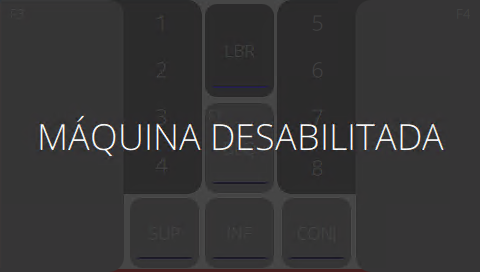
\includegraphics{src/imagesICV/12-KTP400-scout/e-1.png}
\end{figure}
\vspace*{\fill}

\newpage
\thispagestyle{fancy}
\vspace*{40 pt}
\subsection{Tela movimento manual do batedor}
    Ver: \ref{sec:comandosBatedorMovimentoManualGuias} - \nameref{sec:comandosBatedorMovimentoManualGuias}.
\vspace*{\fill}
\begin{figure}[h]
  \centering
  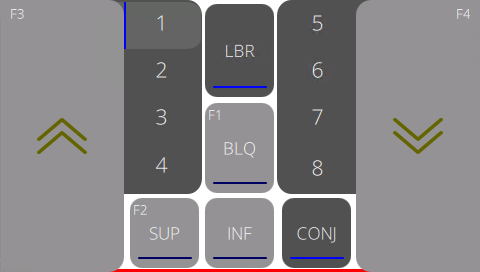
\includegraphics{src/imagesICV/12-KTP400-scout/e-2.png}
\end{figure}
\vspace*{\fill}

\newpage
\thispagestyle{fancy}
\vspace*{40 pt}
\subsection{Tela desvio das guais do batedor}
    Ver: \ref{sec:comandosBatedorAberturaGuias} - \nameref{sec:comandosBatedorAberturaGuias}.
\vspace*{\fill}
\begin{figure}[h]
  \centering
  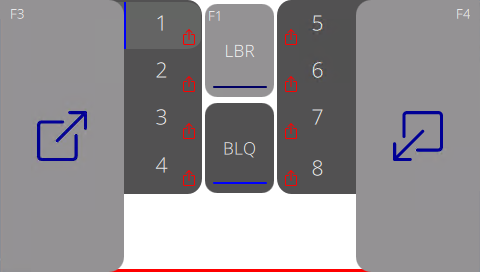
\includegraphics{src/imagesICV/12-KTP400-scout/e-3.png}
\end{figure}
\vspace*{\fill}



